\documentclass[compress,mathserif]{beamer}
\usetheme{sthlm}

%-=-=-=-=-=-=-=-=-=-=-=-=-=-=-=-=-=-=-=-=-=-=-=-=
%        LOADING BEAMER PACKAGES
%-=-=-=-=-=-=-=-=-=-=-=-=-=-=-=-=-=-=-=-=-=-=-=-=

\usepackage{
booktabs,
datetime,
dtk-logos,
graphicx,
multicol,
pgfplots,
ragged2e,
tabularx,
tikz,
wasysym,
multirow,
float,
caption,
subcaption,
amsmath,
mathptmx,
animate
}

\usepackage[scaled=0.9]{helvet}
\usepackage{courier}

\usefonttheme[onlymath]{serif}

\definecolor{mygreen}{RGB}{113, 166, 70}
\definecolor{myblue}{RGB}{68, 140, 185}
\definecolor{myred}{RGB}{217, 98, 55}
\definecolor{mypurple}{RGB}{83, 65, 126}
\definecolor{solviaveis}{RGB}{188, 207, 241}

\pgfplotsset{compat=1.8}

\usepackage[utf8]{inputenc}
\usepackage[portuguese]{babel}
\usepackage[T1]{fontenc}
\usepackage{newpxtext,newpxmath}
\usepackage{listings}

\lstset{ %
language=[LaTeX]TeX,
basicstyle=\normalsize\ttfamily,
keywordstyle=,
numbers=left,
numberstyle=\tiny\ttfamily,
stepnumber=1,
showspaces=false,
showstringspaces=false,
showtabs=false,
breaklines=true,
frame=tb,
framerule=0.5pt,
tabsize=4,
framexleftmargin=0.5em,
framexrightmargin=0.5em,
xleftmargin=0.5em,
xrightmargin=0.5em
}



%-=-=-=-=-=-=-=-=-=-=-=-=-=-=-=-=-=-=-=-=-=-=-=-=
%        LOADING TIKZ LIBRARIES
%-=-=-=-=-=-=-=-=-=-=-=-=-=-=-=-=-=-=-=-=-=-=-=-=

\usetikzlibrary{
backgrounds,
mindmap
}

%-=-=-=-=-=-=-=-=-=-=-=-=-=-=-=-=-=-=-=-=-=-=-=-=
%        BEAMER OPTIONS
%-=-=-=-=-=-=-=-=-=-=-=-=-=-=-=-=-=-=-=-=-=-=-=-=

\setbeameroption{show notes}

%-=-=-=-=-=-=-=-=-=-=-=-=-=-=-=-=-=-=-=-=-=-=-=-=
%        BEAMER COMMANDS
%-=-=-=-=-=-=-=-=-=-=-=-=-=-=-=-=-=-=-=-=-=-=-=-=


%-=-=-=-=-=-=-=-=-=-=-=-=-=-=-=-=-=-=-=-=-=-=-=-=
%
%	PRESENTATION INFORMATION
%
%-=-=-=-=-=-=-=-=-=-=-=-=-=-=-=-=-=-=-=-=-=-=-=-=

\title{Introdução a disciplina}
\subtitle{DCE747 - Inglês Técnico}
%\date{\small{\jobname}}
\author{\texttt{Iago Carvalho}}
\institute{\texttt{Departamento de Ciência da Computação}}

\hypersetup{
pdfauthor = {Iago A. Carvalho},      
pdfsubject = {Pesquisa Operacional},
pdfkeywords = {},  
pdfmoddate= {D:\pdfdate},          
pdfcreator = {WriteLaTeX}
}

\begin{document}

\begin{frame}
\titlepage

\end{frame}

%% --------------------------------------------------------

\begin{frame}{Inglês técnico?}

Inglês técnico também é chamado de inglês instrumental em alguns lugares

\vspace{0.5cm}

É um inglês focado no lado profissional
\begin{itemize}
    \item Normalmente direcionado a uma disciplina ou a uma área do conhecimento
\end{itemize}

\vspace{0.5cm}

No nosso caso, vamos ver um inglês focado em computação!

\end{frame}

\section{Pra quê isso vai servir na minha vida?}

%% --------------------------------------------------------

\begin{frame}{Pra quê isso vai servir na minha vida?}

\centering 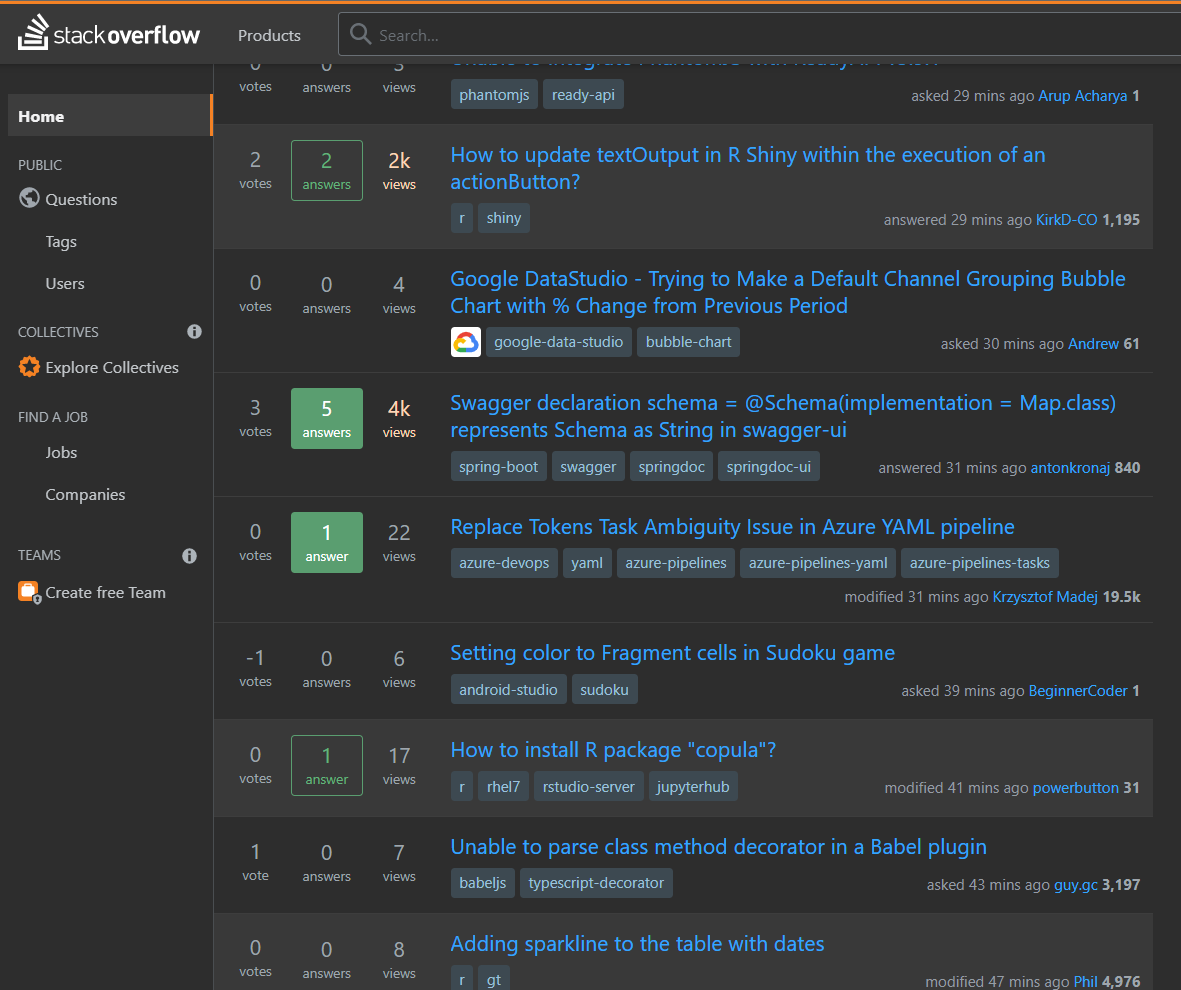
\includegraphics[width=\textwidth]{images/so.png}
\end{frame}

%% --------------------------------------------------------

\begin{frame}{Pra quê isso vai servir na minha vida?}

\centering 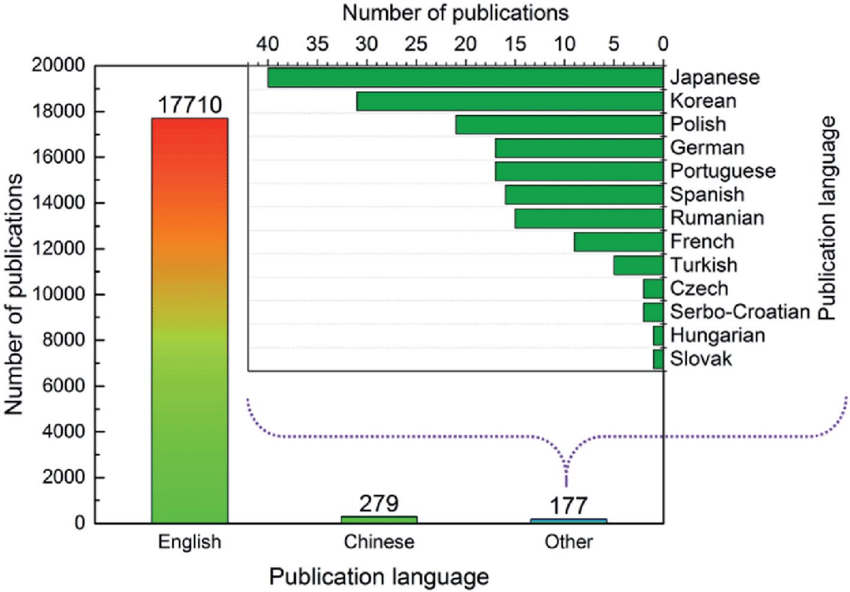
\includegraphics[width=\textwidth]{images/papers_ingles.png}
\end{frame}

%% --------------------------------------------------------

\begin{frame}{Avaliações}

Sem provas! Mas com muito trabalho

\vspace{0.25cm}

Um seminário (20 pontos)
\begin{itemize}
    \item Grupos pequenos (2 ou 3 pessoas)
    \item Um seminário durante o semestre
    \item Seminários distribuídos durante toda a disciplina
    \item Um texto em inglês escolhido a cada semana
\end{itemize}

Resumos de artigos (30 pontos)
\begin{itemize}
    \item Todos devem fazer resumos dos textos apresentados nos seminários
    \item Existem 11 seminários
    \begin{itemize}
        \item Mas só será obrigatório a realização de 8 resumos
        \item Vocês podem pular dois, sem prejuízo de nota
    \end{itemize}
\end{itemize}

\end{frame}

%% --------------------------------------------------------

\begin{frame}{Avaliações}

Exercícios teóricos (20 pontos)
\begin{itemize}
    \item Listas de exercícios disponibilizadas no decorrer do semestre
    \item Entrega em dupla
\end{itemize}

\vspace{0.5cm}

Trabalho final (30 pontos)
\begin{itemize}
    \item A decidir
\end{itemize}

\vspace{0.5cm}

Prova final e especial
\begin{itemize}
    \item Conforme regulamentação da UNIFAL
\end{itemize}
\end{frame}

%% --------------------------------------------------------


\begin{frame}{Acompanhamento da disciplina}

A disciplina será gerida (e deverá ser acompanhada) através de um repositório do Github 
\href{https://github.com/iagoac/dce747/}{\beamergotobutton{Link}}

\vspace{0.5cm}

As atividades escritas deverão ser entregues no Moodle

\vspace{0.5cm}

Seminário deverá ser gravado e disponibilizado um \textit{link}

\end{frame}

\end{document}